\newpage
\section{Neural Networks}
A big part of this project revolved around artificial neural networks, which we used to model the distance maps of particular proteins. 
Therefore, in this section, we fully describe these neural networks.

We start by defining Perceptron, as the simplest instance of neural network architecture.
We show how the Perceptron is constructed, initialized and used to model mathematical functions.
Afterwards, we extend this neural network to enable it to model complex functions.
Next, we show how to use these networks to model spatially dependent data, like, for example, pictures.
Finally, we unite these theoretical concepts and reveal how we used them for the protein folding problem.

% Neural networks are machine learning models discovered in  
% In this section, we will present neural networks due to their high importance in the process of protein folding.

% With sufficient size, neural networks are able to learn any mathematical function.
% Their high complexity and flexibility even allows some particular subtypes, like for example recurrent neural networks, to be turing complete.

% The main challenge these systems are facing is in the fact, that they usually need very big datasets to learn the true mapping and training of such models on such big datasets are often infeasible.
% Nevertheless, the amounts of data collected by mankind is increasing and the computational resources are expected to increase as well. 

% Why Neural Networks?


\subsection{The basic architecture of Neural Networks}
Artificial neural networks are machine learning models first discovered in 1958 by psychologist Frank Rosenblatt.
They were heavily inspired by the human nervous system.
The nervous system is composed of small units, called neurons.
These neurons are connected via specialized connections called synapses.
The synaptic connections allow the neurons to send electrochemical signals to communicate with each other.
The strength of these connections regularly adapts to the external stimulation, which often changes the signal pathways and, in turn, influences the resulting reactions of the organism.
This process is commonly called learning.

\begin{figure}
    \centering
    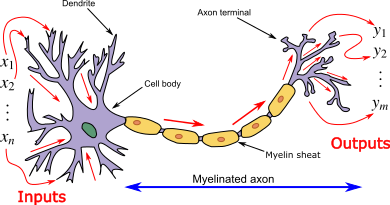
\includegraphics[width=0.5\linewidth]{imgs_andy/biological_neuron.png}
    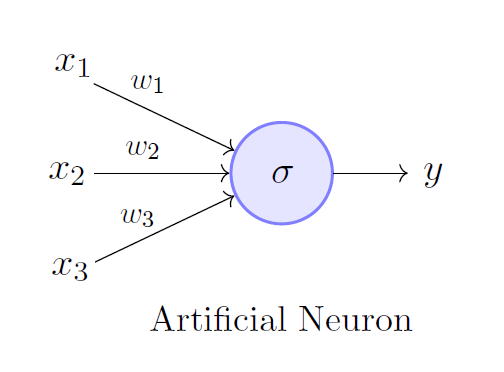
\includegraphics[width=0.5\linewidth]{imgs_andy/artificial_neuron.png}
    \caption{Biological  and Artificial neuron}
    \label{fig:neurons_comparison}
\end{figure}

In artificial neural networks, we simulate this process in a computer.
Similarly to biological neural networks, we have some external stimuli in the form of features $X$.
Furthermore, we provide some desired reaction in the form of labels $Y$, which we would like our network to learn.
The labels are formally related to the features in such a way, that there exists a function $f: X \to Y$.
The learning process then corresponds to finding such function $h$, which approximates the function $f$ the best.
The architecture of the neural network puts some constraints on the set $H$ of all possible functions $h$.

To put the notation in context, let us present an example of the Perceptron architecture.
Imagine we have collected features $X \in R^{n \times d}$, where $n$ is the number of observations and $d$ is the number of predictors.
Based on these features, we would like to build a system capable of distinguishing if datapoint $x_i \in X$ comes from a dog ($y_i = 1$) or a cat ($y_i = -1$).
Our datapoint can, for example, consist of the weight of the animal and the length of the animal's nose.
Given this information, we can construct a Perceptron with 2 input neurons connected to 1 output neuron.
This architecture is depicted in Figure \ref{fig:perceptron}.

\begin{figure}
    \centering
    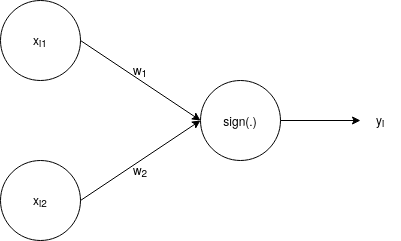
\includegraphics[width=0.5\linewidth]{imgs_andy/perceptron.png}
    \caption{Perceptron}
    \label{fig:perceptron}
\end{figure}

Formally, this architecture models the relation between $X$ and $Y$ according to the Equation \ref{eq:perceptron}. 

\begin{equation}
    y_i = sign(\sum_{j=1}^{d} w_j \cdot x_{ij}) 
    \label{eq:perceptron}
\end{equation}

This modelling approach has 2 significant drawbacks.
First, it assumes the two classes are linearly separable by a hyperplane through the d-dimensional space induced by the predictors.
Second, it assumes the separation hyperplane goes through the centre of mass in the space.
To tackle the latter, we can introduce another parameter $b$, also called bias, to the equation.
The bias can be included as a weight of the edge from the bias neuron, which is a neuron always containing the value 1.
Therefore, we can treat this special case by using the general Equation \ref{eq:perceptron}.
Furthermore, the Equation \ref{eq:perceptron} can be simplified using the vector notation to Equation \ref{eq:perceptron2}.

\begin{equation}
    Y = sign(W \cdot X)
    \label{eq:perceptron2}
\end{equation}

To resolve the problem with linear separability, we can extend our model by using additional layers of neurons.
These additional layers are commonly called hidden layers of the neural network.
In order to be efficient, the hidden layers need to apply some non-linear function, usually called activation function.
The function modelled by this new network is of the form

\begin{equation}
    Y = sign(W_2 \cdot a(W_1 \cdot X)),
    \label{eq:perceptron3}
\end{equation}

where $a$ is the activation function and $W_l, l \in {1, 2}$ are the weights of the connections corresponding to transition from layer $l-1$ to layer $l$.

There is many possibilities for the activation function and the choice of it usually depends on the particular goal in mind.
% from here it feels sloppy
Some of the most commonly used activation functions are:

\begin{itemize}
    \item $\text{Identity}(x) = x$
    \item $\text{Tanh}(x) = \frac{\exp(x) - \exp(-x)}{\exp(x) + \exp(-x)}$
    \item $\text{Sigmoid}(x) = \frac{1}{1 + \exp(-x)}$
    \item $\text{HardTanh}(x) = \begin{cases}
             1 & \text{ if } x > 1 \\
             x & \text{ if } 1 \geq x \geq -1 \\
            -1 & \text{ if } x < -1 \\
          \end{cases}$
    \item $\text{ReLU}(x) = \max(0, x)$
    \item $\text{ELU}(x) = \max(0,x) + \min(0, \alpha * (\exp(x) - 1))$
    \item $\text{Softmax}(x_{i}) = \frac{\exp(x_i)}{\sum_j \exp(x_j)}$
    \label{list:activations}
\end{itemize}

% identity
% softmax
% tanh(x) = 2*sigmoid(2x) -1

% impressive source
% https://ml-cheatsheet.readthedocs.io/en/latest/activation_functions.html
Probably the first non-linear function to consider would be the sign function, since we already used this function in the output layer of the single-layer Perceptron.
Unfortunately, this function has a derivative 0 almost everywhere, with the exception of $x=0$ where it is non-differentiable and discontinuous.
These properties complicate the process of learning and therefore this function is rarely used during the training of the model.
To address these issues, researchers used hyperbolic tangents in the past as the smooth alternative to the sign function, sometimes scaling it to sigmoid function, which can be interpreted in probabilistic manner.
Unfortunately, these functions, although differentiable everywhere, often provide quite small gradients.
This creates a problem commonly called vanishing gradient.
% which we will discuss later in the section
Recently, a solution to this problem was proposed in the form of using Hard Hyperbolic Tangent (HardTanh) or the Rectified Linear Unit (ReLU).
These piecewise activation functions provide a gradients of 0 or 1, depending on the input values.
% dying ReLu problem
Finally, Exponential Linear Unit (ELU) is an improvement of the ReLU function which we use in this project. 
\subsubsection{Activation functions on output layer}
Until this point, we considered only the classification task with two classes.
However, it is possible to extend neural networks to much more different tasks at hand.
One of the possible extensions is the regression task, where our response is some numeric value $Y \in R^n$.
In these settings, we could use the Identity function on the output layer.
The error function, which we want to minimize would be an ordinary least squares. 

Another of the possible extensions is the multiclass classification task, where we want to learn to distinguish more classes.
In this case, we usually encode our output with one-hot-encoding.
For example, consider classification to 3 classes.
In this case, we can encode the labels as follows:
\begin{itemize}
    \item $1 \to (1, 0, 0)$ 
    \item $2 \to (0, 1, 0)$
    \item $3 \to (0, 0, 1)$
\end{itemize}
To enable our network to learn this relation, we use the output layer with 3 output neurons.
In theory, we could just use the Identity function and select the highest value as the predicted class, but in practice the Softmax function is often used.
The Softmax function is defined as:

\begin{equation}
    \text{Softmax}(x_{i}) = \frac{\exp(x_i)}{\sum_j \exp(x_j)}
\end{equation}

and it has some very nice properties.
Firstly, it maps the real-valued outcome to the interval $[0, 1]$.
Secondly, the sum of the outcome is always 1.
To be able to optimize a network with this output, we use the negative log likelihood loss.

\begin{equation}
    \ell(x, y) = \sum_{n=1}^N \frac{1}{\sum_{n=1}^N w_{y_n}} l_n 
\end{equation}

\subsubsection{Training of the neural networks}
The training of the neural networks refers to the learning process.
In neural networks, this is done by adjusting the weights $W$ in such a way that the relationship between input $X$ and output $Y$ is approximated as well as possible.
To be able to evaluate the performance of the current network, we need to define loss function.
This function gets the predicted output $\hat{Y}$ and the real output $Y$ and evaluates the error made during the prediction.
Some commonly used loss functions are, for example, Mean Squared Error (MSE) and the Negative Log-Likelihood.
The Mean Squared Error is mainly used in regression setting, when we want to predict a continuous value.
It is defined by equation \ref{eq:MSE}.

\begin{equation}
    \ell(\hat{Y}, Y) = \text{mean}(L) = \text{mean}(l_1,\dots,l_N), 
    \text{where} l_n = (\hat{Y}_n - Y_n)^2
    \label{eq:MSE}
\end{equation}

The Negative Log-Likelihood is used for classification purposes with C classes.
It is defined by equation\ref{eq:NLL}.

\begin{equation}
    \ell(\hat{Y}, Y) = \sum_{n=1}^N \frac{1}{\sum_{n=1}^N w_{Y_n}} l_n,
    l_n = - w_{y_n} x_{n,y_n},
    \label{eq:NLL}
\end{equation}

The input to this loss function has to contain log-probabilities of each considered class.
Obtaining log-probabilities from the neural network can be achieved by adding Softmax activation function to the output layer and taking logarithm of the resulting values.

Now, with all parts in place, we can illustrate the training process.
The training of the neural networks is done iteratively.
First, we predict the output values $\hat{Y}$ for our input $X$.
This is done in the forward pass through our neural network.
Afterwards, we calculate the error using the loss function.
Then, we use this error to calculate the gradient with respect to weights.
This is done in the backward pass through our neural network.
The weights are then updated in the direction of negative gradient.
The process is then repeated, until convergence is achieved.

This training process is also referred as Gradient Descent and we provide the algorithm in the Box \ref{alg:gd}.

\begin{algorithm}
\caption{Gradient Descent}
\label{alg:gd}
\begin{algorithmic}[1]
\State $w \gets \textit{initialize}$
\Repeat
\State $\hat{Y} = \textit{predict(X, w)}$
\State $w = w - \alpha * \nabla_w E_{in}(\hat{Y}, Y)$
\Until{convergence}
\end{algorithmic}
\end{algorithm}

Although this algorithm provides a solid basis to analyze the learning process, it is usually too slow to be used in practice.
This is mainly caused by the need to calculate the predictions across all the datapoints in the training dataset.
Since nowadays the training datasets tends to be very big a modification to this algorithm was proposed.
Instead of using all the datapoints from training dataset, the error is just estimated with one point.
This is what is called the Stochastic Gradient Descent and it was one of the most significant steps in adopting the neural networks in a broad range of tasks.

The time complexity of the Gradient Descent is $\mathcal{O}(n\log{\frac{1}{\epsilon}})$, where $n$ is the number of datapoints in the training dataset and $\epsilon$ is how far away from the minimum we want to end up.
As we can see, the $n$ factor in this time complexity is very significant when the dataset is huge.
Because the Stochastic Gradient Descent uses just one datapoint to estimate the gradient, it makes noisy estimates, which might not be in the optimal direction, but it is able to make those estimates much more quickly.
The time complexity of this method is $\mathcal{O}(1\cdot\frac{1}{\epsilon})$.

In practice, we prefer to use more datapoints than one during the training to estimate the gradient.
This is called the Mini-Batch Stochastic Gradient Descent and it presents a middle-ground option between the two extremes.
The estimates of the gradient are not as noisy as during the SGD and the time to compute the gradient is also significantly reduced. 

\subsubsection{Parameter initialization}
Another important aspect of the neural networks is their parameter initialization.
A naive solution would be to initialize them to 0 and let the network learn the true weights.
Unfortunately, this naive solution would be a terrible one, because it would cause the neural network to update all the weights the same way.
Therefore, we usually initialize the weights to some random weights.
This ensures to break the symmetry during the learning and allows to update the weights efficiently.

Another thing to consider is the magnitude of these newly initialized weights.
Too big or too small values can cause numerical issues during the training due to limitations of float number representation in computers, which are inherently discreet systems.
Initializing the weights to sample from Uniformly distributed values from interval [0, 1] or from Normal distributed values with mean 0 and standard deviation 1 usually works fine for smaller neural networks, but might cause numerical problems when the number of input connections and the number of output connections is big.
Therefore, an improved aproaches, which take number of incomming and outgoing connections, were proposed.
First approach is the Glorot initialization \cite{glorot2010understanding}.
In this initialization, the weights are sampled either from an Uniform distribution from interval [$-a, a$] or from Normal distribution with mean 0 and standard deviation $a$, where parameter $a$ is defined as:

\begin{equation}
    a = \text{gain} \times \sqrt{\frac{6}{\text{fan\_in} + \text{fan\_out}}}
\end{equation}

Another approach is the He initialization \cite{he2015delving}.
This initialization is very similar to Glorot initialization and the only difference is in the calculated value of the parameter.
In the case of Uniform distribution, the boundary parameter is calculated by

\begin{equation}
    \text{bound} = \text{gain} \times \sqrt{\frac{3}{\text{fan\_mode}}},
\end{equation}

and in the case of Normal distribution, the standard deviation parameter is calculated by

\begin{equation}
    \text{std} = \frac{\text{gain}}{\sqrt{\text{fan\_mode}}}.
\end{equation}
% this needs more explanation

\subsection{Convolutional Neural Networks}
Convolutional neural network (CNN) is a special type of neural network designed to work with data with a strong spatial dependence.
One canonical example of such data are images.
The strong spatial dependence in the image data is demonstrated by the fact that often the regions close to each another exhibit the same values of the pixel colors.
Another important feature of the image data is the translational invariance, meaning that an object moved from one position in the picture to another position is still identifiable.

A basic operation in the convolutional neural networks is the convolution.
The convolution operation is inspired by the experiments on cat's visual cortex performed by Hubel and Wiesel \cite{hubel1959receptive}.
Here, the biological neurons are divided into small regions which differ in sensitivity towards the stimuli from different regions of visual field.
Furthermore, the sensitivity of different regions varies with the different shape and orientation of the observed objects.
For example, a vertical lines in the visual field can activate some regions of the biological neurons and horizontal lines can activate different regions of the biological neurons.
The regions are then connected in hierarchical fashion, which allows the deeper regions to recognize for example squares.

% add: locality 
Convolutional neural networks are using similar principles to extract and encode an important features of presented image.
From the computational point of view, CNNs are neural networks heavily regularized by the number and location of connections.
They perform exceptionally well on image classification tasks, recently achieved human-level performance on ImageNet dataset.
The ImageNet dataset is the benchmark dataset used in ImageNet Large Scale Visual Recognition Competition (ILSVRC), which is annual competition hugely contributing to the development and application of neural networks.
% add:
% different architectures, with just minor changes
% some notable winners - LeNet, AlexNet, 

\subsubsection{Convolution layer}
% add: CNN defined as neural netowkrs with at least one convolutional layer 
Convolution layer is the characteristic unit of the Convolutional Neural Network.
It applies the Kernel to the data to transform the input to the output.
The Kernel is a small grid with trainable parameters.
To illustrate how to apply such a Kernel to the data let us imagine a Kernel $K$ with the size $3 \times 3$.
In this example, we will apply this to an image $I$ of size $5 \times 5$ pixels, where each pixel contains one numerical value, representing the brightness of the pixel.
First we will apply the Kernel to the image at position $(0, 0)$.
This means, we will do element-wise multiplication between the Kernel and the part of the Image from position 0 to position 3 on x-axis and from position 0 to position 3 on y-axis.
Afterwards, we will sum all the products of the multiplication to get a first result of the convolution process with position (0, 0).
Then, we will move the Kernel by one pixel to the right.
Here, we will perform the same operation, with the only difference that the part of the Image used in this convolution will start at position 1 on the x-axis and 0 on the y-axis.
The result of this convolution will be assigned to the position (1, 0) as well.
We continue the operation by shifting the Kernel to the right until we reach the end if the Image.
Afterwards, we will shift the Kernel by one pixel down and start the same process of convolution on this row.
This is repeated until we slide through all possible rows and columns of the Image grid.
The convolution operation is visualized in Figure \ref{fig:convolution}.

\begin{figure}
    \centering
    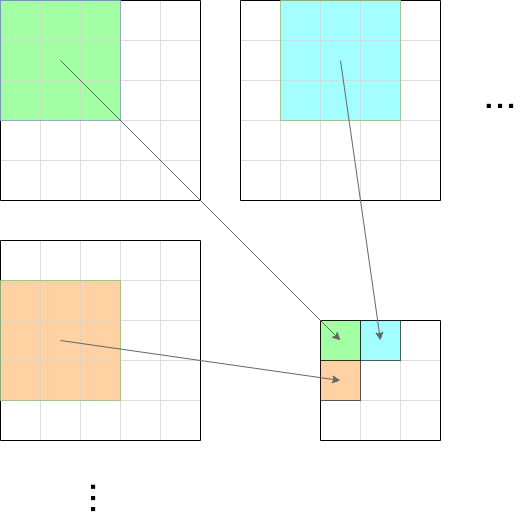
\includegraphics[width=\linewidth]{imgs_andy/convolution.png}
    \caption{Convolution operation}
    \label{fig:convolution}
\end{figure}

% padding
An important observation in this case is that the convolution operation reduces the size of the image by default.
This behaviour is usually not desirable, because it might lead to loss of information at the edge of the image.
Fortunately, it can be easily corrected by using a padding.
Using the padding results in adding some number of pixels, usually containing zeros, to the edge of the image.
In our example, we could extend the Image from $5 \times 5$ to $7 \times 7$ by adding zeros around it.
This would ensure, that the dimensionality of the picture stays the same after convolution.

% half-padding
The size of the padding mainly depends of the size of the selected kernel.
Some of the most used kernel sizes are $3 \times 3$, $5 \times 5$ and $7 \times 7$, with their corresponding paddings $1$, $2$ and $3$.
In general, the padding preserving the size of the image is of size $(F_q - 1)/2$ pixels wide.
This type of padding is also called half-padding, because almost half of the kernel is sticking out of the original image at the edges.

% valid padding
Using the half-padding usually works better in experiments than using no padding, which is sometimes also referred as valid padding.
The intuition behind this remark is that valid padding tends to under-represent the information at the borders in comparison with the central pixels of the image.
Due to these disadvantages of the valid padding, it is rarely used in practice and most of the architectures tend to use the half-padding.

% full padding
Another type of padding is the full-padding.
In this case, we will pad the image with border of $F_q - 1$ zeros wide.
This padding allows almost the full kernel to stick out of the image.
One interesting remark about this type of padding is that every pixel of the original image is covered same number of times.
Furthermore, this padding increases the dimensions of the image by $F_q - 1$.
To illustrate the reason why, let us consider the image of size $(W, H)$.
This image will be padded by $F_q - 1$ from all sides, therefore the size of the padded image will be $(W + 2\cdot(F_q - 1), H + 2\cdot(F_q - 1))$.
After convolution, this padded image will be reduced to $(W + F_q - 1, H + F_q - 1)$, therefore it is bigger by $F_q - 1$ in every dimension in comparison to the original image.
This fact is sometimes used in "reverse" convolution layers, which are mainly used in different autoencoder architectures.

\subsubsection{Strides}
Until now, we considered two parameters of a convolution layer - kernel size and padding.
Another parameter sometimes used in convolution layers is stride.
The stride correspond to the shift by which we move the kernel along the axis.
In the previous example, we used the stride of $1$.
Using the bigger values for stride $S$ has an effect of reduction of the dimension of the image by a factor of approximately $S$. 
To clarify how this is done, let us consider the movement on the x-axis in the previous example.
There, we started at the position 0, then continued with position 1, followed by position 2 and so on.
This can also be written as a sequence $0\cdot S, 1\cdot S, 2\cdot S\dots$ with the stride parameter $S = 1$.
By increasing the stride parameter to 2, we would get a sequence $0\cdot2, 1\cdot2, 2\cdot2\dots = 0, 2, 4\dots$.
This is also shown in Figure \ref{fig:stride}

\begin{figure}
    \centering
    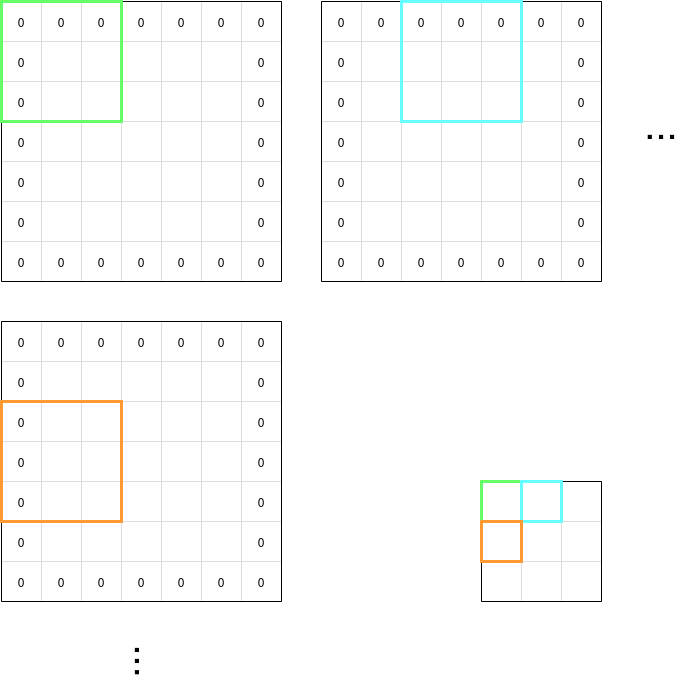
\includegraphics[width=0.6\linewidth]{imgs_andy/stride.png}
    \caption{Convolution with half-padding and stride 2}
    \label{fig:stride}
\end{figure}

It is noteworthy, that increased stride reduces the dimensions of the image.
This effect is even stronger than reduction of the dimensions by valid padding, but it does not suffer by under-representing data closer to the border.
In general, it reduces the size of the image according to the Equation \ref{eq:stride}, where $L_1$ is the length of the dimension when using the stride $S=1$ and $S$ is the used stride.

\begin{equation}
    L_S = \floor*{L_1 / S}
    \label{eq:stride}
\end{equation}

Sometimes, this reduction is even used as an advantage, especially, when the resolution of the image is too high.
It can also help to reduce over-fitting or in cases, when the memory is constrained.
Another remark is that the stride increases the receptive field of the consequent convolutions.
This allows the consequent convolutions to capture more complex features in the deeper layers.
A similar function is performed by another characteristic layer of Convolutional Neural Networks presented in the following part.

\subsubsection{Pooling layer}
Similarly to the Convolution layers, Pooling layers operate on small regions of the Image.
There are two main difference between these two types of layers.
First difference is that the pooling layer usually uses the stride parameter $S$ of the same value than the size of the kernel in that particular direction.
The second difference is that the pooling layer does not use the dot product.
The most common practice is to take the maximum of the entry-wise product.
This is referred as max-pooling.
Additionally, pooling can use any other function, which takes the matrix of entry-wise products and returns a single number, like for example average.
These other functions are rarely used, mainly due to their worse performance in practice. 

The main purpose of the pooling layers in Convolutional Neural Networks is to increase the receptive field in the consecutive layers, while decreasing the spatial size.
A similar effect can be accomplished with strided convolutions, which sometimes makes pooling layers unnecessary.
Nevertheless, the effect of max pooling can not be exactly replicated due to the max operation.

\subsubsection{Dilated convolutions\cite{yu2015multi}}
% https://towardsdatascience.com/review-dilated-convolution-semantic-segmentation-9d5a5bd768f5
As we saw in previous examples, the standard convolutions take into account a region of the input image and perform the convolution operation with the kernel.
This region usually consists of a few consecutive pixels in the x-axis and y-axis.
A relatively recent innovation is to consider as a region pixels separated by a few skipped pixels.
This is shown in the Figure \ref{fig:dilated_conv}.

\begin{figure}
    \centering
    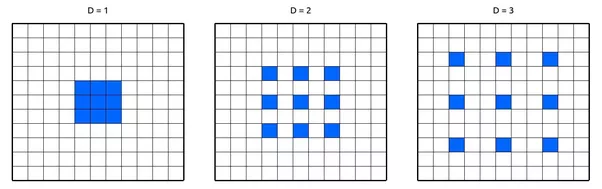
\includegraphics[width=\linewidth]{imgs_andy/dilated_conv.png}
    \caption{Dilated convolutions}
    \label{fig:dilated_conv}
\end{figure}

This is called dilated convolutions and effectively it increases receptive field of the convolution operation.
Formally, the output of convolution at position $i, j$ of input map can be calculated as:

\begin{equation}
    \text{OUT}_{i,j} = \sum_{k=0}^{K-1} \sum_{l=0}^{K-1} \text{IN}_{i+(k \cdot D),j+(l \cdot D)} \cdot \text{KERNEL}_{k, l},
\end{equation}

where $K$ is the kernel size and D is the dilation.

% local connectivity - the neuron will be connected only to small number of neurons in the previous layer, which are close together
% part of the image that the neuron is connected to is called receptive field
% The receptive field is defined as the region in the input space that a particular CNN’s feature is looking at (i.e. be affected by)
% https://medium.com/mlreview/a-guide-to-receptive-field-arithmetic-for-convolutional-neural-networks-e0f514068807

\subsubsection{Convolutions through multiple channels}
% basic principle
Up to this point, we have considered only convolutions on maps with only one channel.
Examples of such maps are for instance gray scale images, where each grid entry contains one number representing the intensity of light in that particular pixel.
However, commonly the images we want to process consist of pixels with 3 different channels.
Such images can then be represented in a 3-dimensional tensor of $W \times H \times C$, where $W$ is the width of the picture in pixels, $H$ is the height of the picture and $C=3$ is the depth used to store intensities of 3 basic colors - red, green and blue. 

In this case, the convolution is performed similarly to the convolution in the simple case, only now our kernel is of size $K \times K \times 3$.
The computation of the output value is shown in the Equation \ref{eq:conv_channels}.

\begin{equation}
    \text{OUT}_{i,j} = \sum_{k=0}^{K-1} \sum_{l=0}^{K-1} \sum_{m=0}^{C-1} 
        \text{IN}_{i+k,j+l, m} \cdot \text{KERNEL}_{k, l, m}.
    \label{eq:conv_channels}
\end{equation}

Often, it is desired to transform the input with multiple channels to output with multiple channels, where the output channels capture different features of the Image.
This is done using multiple kernels where each kernel produces a single map of some specific features.
For example, we can have one kernel which is able to detect edges of the objects in the image and another kernel which is able to detect texture of the objects.
To incorporate these options, PyTorch framework allows to initialize the convolution layers with parameters $\text{in\_channels}$, $\text{out\_channels}$, $\text{kernel\_size}$, $\text{padding}$, $\text{stride}$, $\text{dilation}$.










% 1X1 convolution

% reduction of the parameters using the 1X1 convolution

\subsection{Residual Neural Networks}
    
\subsection{AlphaFold}

\newpage